%% ----------------------------------------------------------------
%% Chapter_4.tex
%% ----------------------------------------------------------------
\chapter{Project Description}
\label{Chapter:Description}

\section{SOFTWARE MODEL}
EduFeedback AI follows a layered client-server architecture to make the system easier to manage, scale, and improve over time. The overall design is divided into four logical layers, with each layer handling a specific role in the system. This clear separation of responsibilities helps keep the system well-organized and reduces dependency between components. As a result, updates or improvements can be made to one part of the system without disrupting others, which supports long-term maintenance and future expansion.

The application layer is the part of the system that handles most of the working logic. It connects what the user does on the website with what happens in the backend. This layer checks who the user is, what role they have, and whether they are allowed to access a particular feature. It also makes sure that the data sent by users is valid before moving it further. When alumni submit surveys or faculty members provide course-related feedback, this layer manages how the information flows through the system. Keeping these rules in one place helps in making small changes later without affecting the full system. The data analytics layer is mainly responsible for understanding the information collected from users. Most of the feedback received is in text form and cannot be directly used for analysis. This layer processes such data and looks for useful patterns and meanings in it. It compares alumni feedback, job-related information, and course details to find how well the curriculum matches industry needs. Based on this comparison, the system highlights areas where skills are lacking and subjects that need improvement. This layer is kept flexible so that better analysis methods or new data sources can be added in the future if required.

The data analytics layer encapsulates all intelligence-driven components of the system. This layer integrates Natural Language Processing and machine learning models to analyze unstructured and semi-structured data. NLP techniques such as TF-IDF and BERT-based embeddings are employed to extract meaningful features from alumni feedback, job descriptions, and curriculum documents. Similarity computation algorithms quantify curriculum-industry alignment, while scoring models compute metrics such as the Skill Gap Index and Course Relevance Score. This layer is designed to be extensible, allowing future inclusion of advanced predictive models and external labor market datasets.

The data layer functions as the persistent storage foundation of the system. A relational database management system is used to store structured entities including user profiles, alumni career data, skill usage records, course relevance ratings, CO attainment reports, and generated analytics results. Data normalization and relational integrity constraints are enforced to ensure consistency, accuracy, and efficient query processing. This layer supports both transactional operations and analytical queries required by the dashboard and reporting components.

Overall, the layered client-server architecture enables EduFeedback AI to achieve high cohesion within modules and low coupling across layers. Such an architectural design enhances system scalability, facilitates maintenance and future upgrades, and ensures reliable performance when handling growing volumes of academic and alumni data. This design choice aligns with best practices in enterprise software development and supports the long-term adaptability of the proposed system.

\section{SOFTWARE REQUIREMENTS SPECIFICATION (SRS)}

\subsection{INTRODUCTION}
EduFeedback AI is an AI-driven academic analytics system designed to assess curriculum relevance by integrating alumni career outcomes, faculty feedback, and curriculum content. The system aims to support Outcome-Based Education (OBE) by providing quantitative and qualitative insights that assist academic administrators in curriculum evaluation and continuous improvement. This SRS document outlines the functional and non-functional requirements, system constraints, and expected performance characteristics of the proposed system.

\subsection{GENERAL DESCRIPTION}
EduFeedback AI is a web-based, client-server application developed using a layered architecture. The system supports multiple user roles, including alumni, faculty members, and administrators. Alumni provide post-graduation career data through structured surveys, faculty submit CO attainment reports, and administrators analyze aggregated insights via dashboards. The system incorporates Natural Language Processing and machine learning techniques to extract skills from unstructured text, compare them with curriculum topics, and generate curriculum refinement recommendations. The software is designed to be modular, scalable, and extensible.

\subsection{FUNCTIONAL REQUIREMENTS}
The system shall provide the following functionalities:
\begin{itemize}
    \item The system shall allow alumni to register, authenticate, and submit career outcome surveys.
    \item The system shall enable alumni to update their employment and skill-related information periodically.
    \item The system shall allow faculty members to log in and upload CO attainment reports and qualitative feedback.
    \item The system shall accept syllabus documents in text or document format for analysis.
    \item The system shall preprocess textual data using NLP techniques.
    \item The system shall extract curriculum topics and industry skills using NLP models.
    \item The system shall compute Skill Gap Index and Course Relevance Score.
    \item The system shall generate automated curriculum improvement recommendations.
    \item The system shall provide an admin dashboard with data visualization and reporting capabilities.
    \item The system shall support export of analytical reports in PDF and spreadsheet formats.
\end{itemize}

\subsection{INTERFACE REQUIREMENTS}
\textbf{User Interface}
\begin{itemize}
    \item Web-based interfaces accessible via standard browsers.
    \item Role-specific dashboards for alumni, faculty, and administrators.
    \item Responsive design to support multiple screen sizes.
\end{itemize}

\textbf{Hardware Interface}
\begin{itemize}
    \item Runs on standard desktop or laptop systems with internet connectivity.
\end{itemize}

\textbf{Software Interface}
\begin{itemize}
    \item Relational Database Management System (MySQL/PostgreSQL).
    \item NLP libraries such as scikit-learn and transformer-based models.
    \item RESTful APIs for communication between frontend and backend modules.
\end{itemize}

\subsection{PERFORMANCE REQUIREMENTS}
\begin{itemize}
    \item The system shall handle concurrent access from multiple users without degradation in performance.
    \item Response time for survey submission and dashboard queries shall not exceed acceptable web application limits.
    \item Data processing and skill-matching operations shall complete within defined time constraints for moderate data volumes.
    \item System uptime shall be maintained at a high level during academic sessions.
\end{itemize}

\subsection{DESIGN CONSTRAINTS}
\begin{itemize}
    \item The system shall be developed using open-source frameworks and tools.
    \item Data privacy and access control constraints shall be enforced.
    \item The design shall adhere to OBE, NAAC, and NBA documentation requirements.
    \item The system must be deployable on standard institutional infrastructure.
\end{itemize}

\subsection{NON-FUNCTIONAL ATTRIBUTES}
\textbf{Reliability}: The system shall ensure reliable data storage and retrieval, with safeguards against data loss.
\textbf{Security}: Role-based authentication and authorization. Secure handling of user credentials. Restricted access to sensitive academic and alumni data.
\textbf{Usability}: Simple and intuitive user interfaces. Minimal training required for users.
\textbf{Maintainability}: Modular design enables easy updates and enhancements. Clear separation between data, logic, and presentation layers.
\textbf{Scalability}: Ability to accommodate increasing numbers of users and data volume.

\section{FUNCTIONAL SPECIFICATION}

\subsection{TEXT PREPROCESSING PIPELINE}
Before features are extracted and embedded, raw textual data from alumni surveys and syllabus PDFs must be uniformly processed.

\textbf{Input Corpora}
\begin{enumerate}
    \item \textbf{Alumni Free-Text}: Extracted from survey fields (e.g., job\_responsibilities, tools\_software, skills\_acquired\_after\_graduation).
    \item \textbf{Syllabus PDF Text}: Extracted via pdfplumber (Unit headers, Learning Objectives, Topic breakdowns).
\end{enumerate}

\textbf{Processing Steps (spaCy)}
\begin{enumerate}
    \item \textbf{Lowercasing}: Convert all text to lowercase for uniformity.
    \item \textbf{Tokenization}: Split sentences into individual word tokens.
    \item \textbf{Stopword Removal}: Remove standard English stopwords and a custom academic lexicon. (e.g. {"unit", "module", "chapter", "semester", "course", "subject", "study", "learn", "understand", "basic", "introduction", "advanced"})
    \item \textbf{Lemmatization}: Reduce words to their dictionary root (e.g., "modules" $\rightarrow$ "module", "implementing" $\rightarrow$ "implement").
    \item \textbf{Entities \& N-grams}: Extract unigrams and bigrams via sliding window arrays to preserve context (e.g., "machine learning", "data structures").
\end{enumerate}

\subsection{Feature Extraction \& Embedding Models (Hybrid Ensemble)}
The system employs a Hybrid/Ensemble Feature Representation strategy for text vectorization. Rather than relying on a single traditional Machine Learning algorithm, the pipeline ensembles Statistical Keyword Scoring (TF-IDF) with Deep Contextual Embeddings (BERT). This hybrid approach ensures both rare, highly-specific technical keywords (captured by TF-IDF) and broad, conceptually similar phrases (captured by BERT) are mathematically captured.

The following Python modules and libraries strictly manage this ensemble pipeline:
\begin{itemize}
    \item \textbf{spaCy (en\_core\_web\_sm model)}: Handles linguistic rules, tokenization, and Named Entity Recognition (NER).
    \item \textbf{scikit-learn}: Powers the TF-IDF vectorization and cosine similarity matrix computations.
    \item \textbf{sentence-transformers}: Interfaces with PyTorch to provide the BERT neural network embeddings.
    \item \textbf{pdfplumber}: Handles the robust structural extraction of text and tables from legacy syllabus PDFs.
    \item \textbf{ReportLab}: Generates the finalized visually robust revised syllabus PDFs.
    \item \textbf{Celery and Redis}: Provide an asynchronous task queue to orchestrate the computationally expensive embedding processes without blocking API requests.
\end{itemize}

\textbf{TF-IDF (TERM FREQUENCY-INVERSE DOCUMENT FREQUENCY)}
Used primarily to determine the statistical importance of words across the entire institution's corpus.
\begin{itemize}
    \item Vocabulary/Max Features: 5000 (tunable).
    \item N-gram range: (1,2)
    \item Sublinear TF Scaling: Enabled to compress term frequency impact.
\end{itemize}

\textbf{BERT SEMANTIC EMBEDDINGS}
Provides deep contextual reasoning. It ensures that synonyms or distinct phrases with similar meanings map to the same vector space.
\begin{itemize}
    \item Model Selected: \texttt{sentence-transformers/all-mpnet-base-v2}
    \item Dimensionality: 768-dimensional vectors.
    \item Hardware Match: Optimized for Apple M3 Max / 36GB memory constraints without requiring heavy quantization.
\end{itemize}

\subsection{MATHEMATICAL MODEL \& SCORING FORMULA’S}
\textbf{COSINE SIMILARITY MATCHING}
The foundational operation to compare an Alumni Skill ($S$) against a Syllabus Topic ($T$) within a Course ($C$).

\[
\text{Similarity}(S, T) = \frac{E(S) \cdot E(T)}{\|E(S)\| \times \|E(T)\|}
\]

Where $E(S)$ is the BERT vector of the extracted skill, $E(T)$ is the BERT vector of the syllabus topic. Result range is [-1, 1], where values closer to 1 indicate exact semantic matches.

\textbf{SKILL GAP INDEX (SGI)}
For a specific skill $S$ reported by alumni, what is the gap in the current course $C$?
First, we find the best-matching topic in the course:
\[
\text{Best Match}(S, C) = \max_{T_i \in C} \; \text{Similarity}(S, T_i)
\]
Then, the Skill Gap Index is computed as:
\[
SGI(S, C) = 1.0 - \text{Best Match}(S, C)
\]
Note: A higher SGI indicates a wider gap.

\textbf{COURSE RELEVANCE SCORE (CRS)}
An aggregate score from 0.0 to 1.0 defining how relevant a specific course is to industry demands.
Case A: Faculty Module Enabled (CO Data Available): 
\[
CRS = (w_1 \times R_{\text{alumni}}) + (w_2 \times M_{\text{skill}}) + (w_3 \times A_{\text{CO}})
\]
Where:
\begin{itemize}
    \item $w_1, w_2, w_3$ = Institution-configured weights where $w_1 + w_2 + w_3 = 1.0$
    \item $R_{\text{alumni}}$ = Average alumni rating normalized to [0,1]
    \item $M_{\text{skill}}$ = Average cosine similarity across targeted skills mapped to the course.
    \item $A_{\text{CO}}$ = Average internal course outcome attainment percentage.
\end{itemize}

\subsection{RECOMMENDATION ENGINE LOGIC}
When a skill gap is identified, the system evaluates the importance and urgency of addressing that gap using a priority score.
\[
\text{Priority Score} = SGI \times P_{\text{mention}} \times W_{\text{recency}}
\]
Where $P_{\text{mention}}$ is Alumni Mention Percentage, and $W_{\text{recency}}$ is Recency Multiplier (1.5 if emerging trend, 1.0 otherwise).

\textbf{CLASSIFICATION RULES}
The AI flags syllabus topics applying the following deterministic thresholds:
\begin{enumerate}
    \item \textbf{Type: ADD (High Demand, Low Coverage)}
    \item \textbf{Type: REDUCE / REVIEW (Low ROI Topics)}
    \item \textbf{Type: OVERHAUL (Severe Misalignment)}
\end{enumerate}

\subsection{SYLLABUS DIFF GENERATION}
During the AI revision process, recommendations (Type ADD/REDUCE/MODIFY) need to be inserted correctly back into the syllabus structure.

\textbf{Topic Insertion Algorithm (For ADDs):} Let $R_{\text{topic}}$ be the recommended industry skill. To determine which Unit it belongs to:
\begin{enumerate}
    \item Compute cosine similarity between $E(R_{\text{topic}})$ and $E(\text{Unit\_Header}_i)$ for all units $i$ in the course.
    \item Assign the new topics to the unit where the similarity is maximized:
\[
\max_i \; \text{similarity}(R_{\text{topic}}, \text{Unit\_Header}_i)
\]
    \item If $\max(\text{similarity}) < 0.30$, propose appending a completely new unit.
\end{enumerate}

The Diff Generator then builds a JSON object marking original strings in red (REDUCE/DELETE) and proposed new strings in green (ADD), paired directly with evidence metrics ($P_{\text{mention}}$ and $W_{\text{recency}}$) to present the Diff view to the administrator.

\section{Design Specification}

\subsection{USE-CASE DIAGRAMS}

\begin{figure}[!htbp]
    \centering
    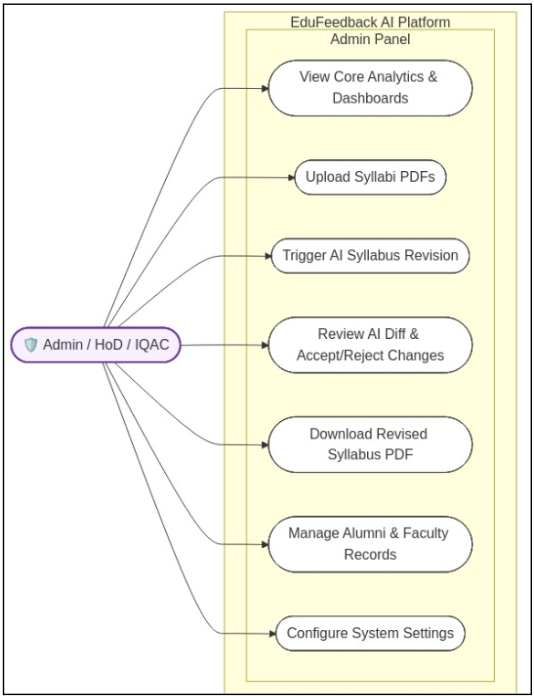
\includegraphics[width=0.65\linewidth, height=0.75\textheight, keepaspectratio]{figures/Chapter_4_Fig/uc_admin.png}
    \caption{Use-case diagram for Admin}
    \label{fig:uc_admin}
\end{figure}

\begin{figure}[!htbp]
    \centering
    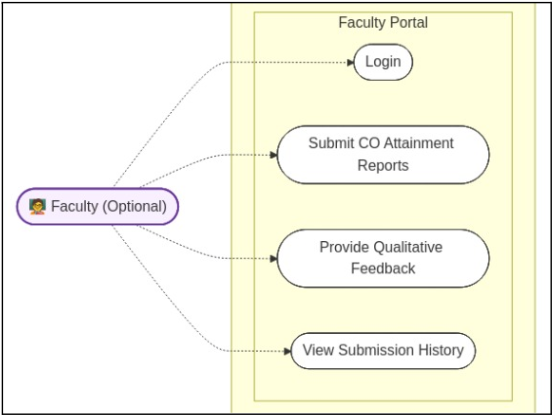
\includegraphics[width=0.65\linewidth, height=0.75\textheight, keepaspectratio]{figures/Chapter_4_Fig/uc_faculty.png}
    \caption{Use-case diagram for Faculty}
    \label{fig:uc_faculty}
\end{figure}

\begin{figure}[!htbp]
    \centering
    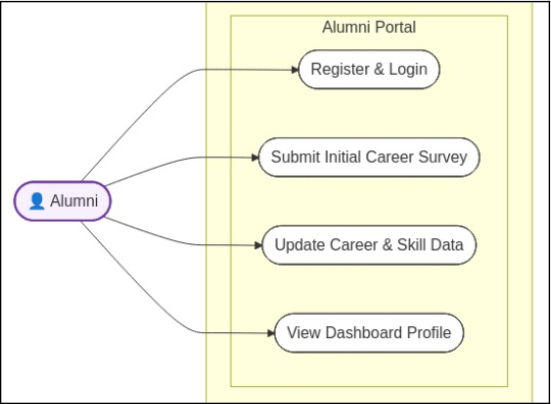
\includegraphics[width=0.65\linewidth, height=0.75\textheight, keepaspectratio]{figures/Chapter_4_Fig/uc_alumni.png}
    \caption{Use-case diagram for Alumni}
    \label{fig:uc_alumni}
\end{figure}

\clearpage
\subsection{DATA FLOW DIAGRAMS (DFD)}

\begin{figure}[!htbp]
    \centering
    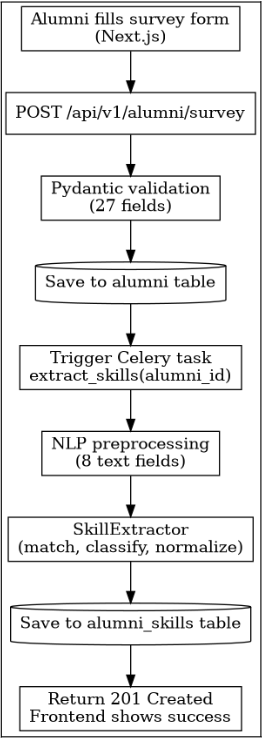
\includegraphics[width=0.75\linewidth, height=0.75\textheight, keepaspectratio]{figures/Chapter_4_Fig/dfd_alumni.png}
    \caption{Alumni Submission Flow}
    \label{fig:dfd_alumni}
\end{figure}

\begin{figure}[!htbp]
    \centering
    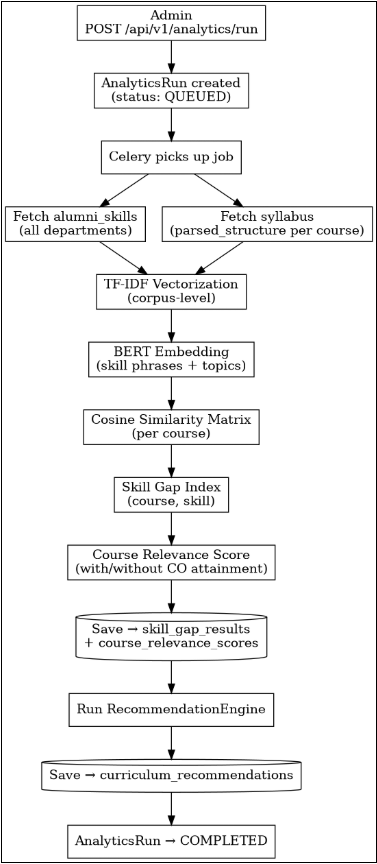
\includegraphics[width=0.75\linewidth, height=0.75\textheight, keepaspectratio]{figures/Chapter_4_Fig/dfd_nlp.png}
    \caption{NLP Analysis Flow}
    \label{fig:dfd_nlp}
\end{figure}

\begin{figure}[!htbp]
    \centering
    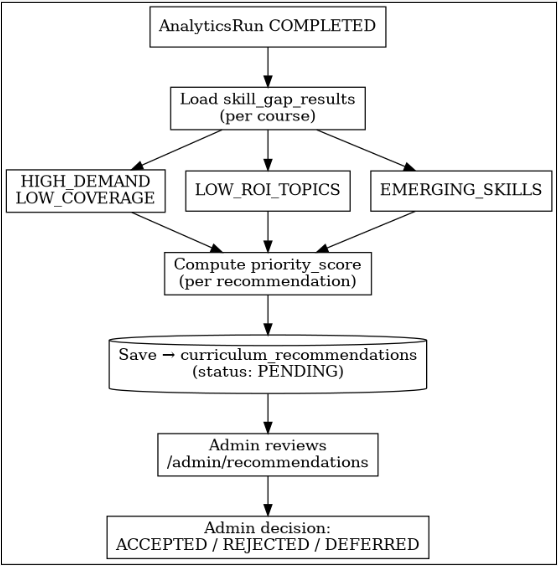
\includegraphics[width=0.75\linewidth, height=0.75\textheight, keepaspectratio]{figures/Chapter_4_Fig/dfd_recommendation.png}
    \caption{Recommendation Generation Flow}
    \label{fig:dfd_recommendation}
\end{figure}

\clearpage

\subsection{DATA DICTIONARY}

\begin{table}[h]
    \centering
    \caption{User Schema}
    \begin{tabular}{|l|l|p{5cm}|}
        \hline
        \textbf{Column} & \textbf{Type} & \textbf{Notes} \\ \hline
        id & UUID PK & \\ \hline
        email & VARCHAR UNIQUE & \\ \hline
        password\_hash & VARCHAR & bcrypt \\ \hline
        role & ENUM & alumni, faculty, admin, superadmin \\ \hline
        department\_id & FK $\rightarrow$ departments & \\ \hline
        full\_name & VARCHAR & \\ \hline
        is\_active & BOOLEAN & Default true \\ \hline
        created\_at & TIMESTAMP & \\ \hline
    \end{tabular}
\end{table}

\begin{table}[h]
    \centering
    \caption{Department Schema}
    \begin{tabular}{|l|l|p{5cm}|}
        \hline
        \textbf{Column} & \textbf{Type} & \textbf{Notes} \\ \hline
        id & UUID PK & \\ \hline
        name & VARCHAR & e.g., "Computer Science Engineering" \\ \hline
        code & VARCHAR & e.g., "CSE" \\ \hline
    \end{tabular}
\end{table}

\begin{table}[h]
    \centering
    \caption{Alumni Survey Form Schema}
    \begin{tabular}{|l|l|p{5cm}|}
        \hline
        \textbf{Column} & \textbf{Type} & \textbf{Notes} \\ \hline
        id & UUID PK & \\ \hline
        user\_id & FK $\rightarrow$ users & \\ \hline
        gender & ENUM & \\ \hline
        degree\_program & VARCHAR & \\ \hline
        department & VARCHAR & \\ \hline
        graduation\_year & INTEGER & \\ \hline
        employment\_status & ENUM & \\ \hline
        job\_role\_designation & VARCHAR & Nullable \\ \hline
        company\_name & VARCHAR & Nullable \\ \hline
        industry\_domain & VARCHAR & Nullable \\ \hline
        work\_mode & ENUM & \\ \hline
        job\_responsibilities & TEXT & NLP source; Nullable \\ \hline
        tools\_software & TEXT & NLP source; Nullable \\ \hline
        skills\_helped\_land\_job & TEXT & NLP source; Nullable \\ \hline
        course\_relevance\_rating & INTEGER & 1-5 \\ \hline
        unused\_subjects & TEXT & NLP source; Nullable \\ \hline
        skills\_missing\_from\_curriculum & TEXT & NLP source; Nullable \\ \hline
    \end{tabular}
\end{table}

\begin{table}[h]
    \centering
    \caption{Alumni Skills Schema}
    \begin{tabular}{|l|l|p{5cm}|}
        \hline
        \textbf{Column} & \textbf{Type} & \textbf{Notes} \\ \hline
        id & UUID PK & \\ \hline
        alumni\_id & FK $\rightarrow$ alumni & \\ \hline
        skill\_name & VARCHAR & Normalized form \\ \hline
        skill\_category & VARCHAR & Programming, Tool, Framework, Domain, Soft Skill \\ \hline
        source\_field & VARCHAR & Which survey field it came from \\ \hline
        is\_post\_graduation & BOOLEAN & True if from skills\_acquired\_after\_graduation \\ \hline
        extracted\_at & TIMESTAMP & \\ \hline
    \end{tabular}
\end{table}

\begin{table}[h]
    \centering
    \caption{Faculty Schema}
    \begin{tabular}{|l|l|p{5cm}|}
        \hline
        \textbf{Column} & \textbf{Type} & \textbf{Notes} \\ \hline
        id & UUID PK & \\ \hline
        user\_id & FK $\rightarrow$ users & \\ \hline
        designation & VARCHAR & \\ \hline
        specialization & VARCHAR & \\ \hline
    \end{tabular}
\end{table}

\begin{table}[h]
    \centering
    \caption{CO Attainment Reports Schema}
    \begin{tabular}{|l|l|p{5cm}|}
        \hline
        \textbf{Column} & \textbf{Type} & \textbf{Notes} \\ \hline
        id & UUID PK & \\ \hline
        faculty\_id & FK $\rightarrow$ faculty & \\ \hline
        course\_id & FK $\rightarrow$ courses & \\ \hline
        academic\_year & VARCHAR & \\ \hline
        semester & INTEGER & \\ \hline
        co\_code & VARCHAR & \\ \hline
        direct\_attainment\_pct & FLOAT & \\ \hline
        indirect\_attainment\_pct & FLOAT & \\ \hline
        final\_attainment\_pct & FLOAT & \\ \hline
        remarks & TEXT & Nullable \\ \hline
        submitted\_at & TIMESTAMP & \\ \hline
    \end{tabular}
\end{table}

\begin{table}[h]
    \centering
    \caption{Faculty Feedback Schema}
    \begin{tabular}{|l|l|p{5cm}|}
        \hline
        \textbf{Column} & \textbf{Type} & \textbf{Notes} \\ \hline
        id & UUID PK & \\ \hline
        faculty\_id & FK $\rightarrow$ faculty & \\ \hline
        course\_id & FK $\rightarrow$ courses & \\ \hline
        topics\_to\_add & TEXT & Nullable \\ \hline
        topics\_to\_remove & TEXT & Nullable \\ \hline
        student\_difficulties & TEXT & Nullable \\ \hline
        general\_comments & TEXT & Nullable \\ \hline
        submitted\_at & TIMESTAMP & \\ \hline
    \end{tabular}
\end{table}

\begin{table}[h]
    \centering
    \caption{Courses Schema}
    \begin{tabular}{|l|l|p{5cm}|}
        \hline
        \textbf{Column} & \textbf{Type} & \textbf{Notes} \\ \hline
        id & UUID PK & \\ \hline
        course\_code & VARCHAR UNIQUE & \\ \hline
        course\_name & VARCHAR & \\ \hline
        department\_id & FK $\rightarrow$ departments & \\ \hline
        semester & INTEGER & \\ \hline
        credits & INTEGER & \\ \hline
        is\_active & BOOLEAN & \\ \hline
    \end{tabular}
\end{table}

\begin{table}[h]
    \centering
    \caption{Syllabus Documents Schema}
    \begin{tabular}{|l|l|p{5cm}|}
        \hline
        \textbf{Column} & \textbf{Type} & \textbf{Notes} \\ \hline
        id & UUID PK & \\ \hline
        course\_id & FK $\rightarrow$ courses & \\ \hline
        academic\_year & VARCHAR & \\ \hline
        original\_file\_path & VARCHAR & Path to uploaded PDF \\ \hline
        parsed\_text & TEXT & Extracted plain text \\ \hline
        parsed\_structure & JSONB & Structured: units $\rightarrow$ topics $\rightarrow$ learning objectives \\ \hline
        is\_processed & BOOLEAN & Has NLP been run? \\ \hline
        uploaded\_by & FK $\rightarrow$ users & Admin who uploaded \\ \hline
        uploaded\_at & TIMESTAMP & \\ \hline
    \end{tabular}
\end{table}

\begin{table}[h]
    \centering
    \caption{Institution Settings Schema}
    \begin{tabular}{|l|l|p{5cm}|}
        \hline
        \textbf{Column} & \textbf{Type} & \textbf{Notes} \\ \hline
        id & INTEGER PK & Single row \\ \hline
        faculty\_module\_enabled & BOOLEAN & Default false \\ \hline
        relevance\_weight\_alumni & FLOAT & w1, default 0.50 \\ \hline
        relevance\_weight\_skill\_match & FLOAT & w2, default 0.50 \\ \hline
        relevance\_weight\_co\_attainment & FLOAT & w3, default 0.0 \\ \hline
        gap\_threshold & FLOAT & Min similarity to not be flagged; default 0.40 \\ \hline
        min\_alumni\_mention\_pct & FLOAT & Min \% for skill to qualify for gap analysis; default 0.10 \\ \hline
        updated\_at & TIMESTAMP & \\ \hline
    \end{tabular}
\end{table}

\begin{table}[h]
    \centering
    \caption{Skill Gap Results Schema}
    \begin{tabular}{|l|l|p{5cm}|}
        \hline
        \textbf{Column} & \textbf{Type} & \textbf{Notes} \\ \hline
        id & UUID PK & \\ \hline
        course\_id & FK $\rightarrow$ courses & \\ \hline
        skill\_name & VARCHAR & \\ \hline
        skill\_category & VARCHAR & \\ \hline
        max\_similarity\_score & FLOAT & Best cosine match vs. any syllabus topic \\ \hline
        alumni\_mention\_count & INTEGER & \\ \hline
        alumni\_mention\_pct & FLOAT & Out of total alumni \\ \hline
        is\_post\_grad\_skill & BOOLEAN & Emerged after graduation \\ \hline
        gap\_flag & BOOLEAN & True = high demand, low coverage \\ \hline
        analytics\_run\_id & FK $\rightarrow$ analytics\_runs & \\ \hline
        computed\_at & TIMESTAMP & \\ \hline
    \end{tabular}
\end{table}

\begin{table}[h]
    \centering
    \caption{Course Relevance Scores Schema}
    \begin{tabular}{|l|l|p{5cm}|}
        \hline
        \textbf{Column} & \textbf{Type} & \textbf{Notes} \\ \hline
        id & UUID PK & \\ \hline
        course\_id & FK $\rightarrow$ courses & \\ \hline
        relevance\_score & FLOAT & Final weighted composite (0-1) \\ \hline
        alumni\_relevance\_avg & FLOAT & From course\_relevance\_rating \\ \hline
        skill\_match\_score & FLOAT & From cosine similarity avg \\ \hline
        co\_attainment\_avg & FLOAT & NULL if faculty module disabled \\ \hline
        analytics\_run\_id & FK $\rightarrow$ analytics\_runs & \\ \hline
    \end{tabular}
\end{table}

\begin{table}[h]
    \centering
    \caption{Curriculum Recommendations Schema}
    \begin{tabular}{|l|l|p{5cm}|}
        \hline
        \textbf{Column} & \textbf{Type} & \textbf{Notes} \\ \hline
        id & UUID PK & \\ \hline
        course\_id & FK $\rightarrow$ courses & \\ \hline
        recommendation\_type & ENUM & ADD, REDUCE, MODIFY, REVIEW, OVERHAUL \\ \hline
        target\_topic & VARCHAR & \\ \hline
        evidence\_summary & TEXT & \\ \hline
        priority\_score & FLOAT & \\ \hline
        status & ENUM & PENDING, ACCEPTED, REJECTED, DEFERRED \\ \hline
        included\_in\_revision & BOOLEAN & Was it applied to a revised syllabus PDF? \\ \hline
        analytics\_run\_id & FK $\rightarrow$ analytics\_runs & \\ \hline
        generated\_at & TIMESTAMP & \\ \hline
    \end{tabular}
\end{table}

\begin{table}[h]
    \centering
    \caption{Syllabus Revisions Schema}
    \begin{tabular}{|l|l|p{5cm}|}
        \hline
        \textbf{Column} & \textbf{Type} & \textbf{Notes} \\ \hline
        id & UUID PK & \\ \hline
        syllabus\_document\_id & FK $\rightarrow$ syllabus\_documents & \\ \hline
        analytics\_run\_id & FK $\rightarrow$ analytics\_runs & \\ \hline
        diff\_data & JSONB & List of change objects \\ \hline
        revised\_structure & JSONB & Full revised syllabus structure \\ \hline
        revised\_pdf\_path & VARCHAR & Path to generated revised PDF; NULL until finalized \\ \hline
        applied\_changes\_count & INTEGER & \\ \hline
        rejected\_changes\_count & INTEGER & \\ \hline
        created\_by & FK $\rightarrow$ users & Admin who triggered revision \\ \hline
        finalized\_at & TIMESTAMP & When admin downloaded/finalized \\ \hline
    \end{tabular}
\end{table}

\begin{table}[h]
    \centering
    \caption{Analytics Runs Schema}
    \begin{tabular}{|l|l|p{5cm}|}
        \hline
        \textbf{Column} & \textbf{Type} & \textbf{Notes} \\ \hline
        id & UUID PK & \\ \hline
        triggered\_by & FK $\rightarrow$ users & \\ \hline
        status & ENUM & QUEUED, RUNNING, COMPLETED, FAILED \\ \hline
        started\_at & TIMESTAMP & \\ \hline
        completed\_at & TIMESTAMP & \\ \hline
        alumni\_count & INTEGER & Snapshot of data volume at run time \\ \hline
        faculty\_data\_included & BOOLEAN & Whether CO data was used in this run \\ \hline
        error\_log & TEXT & Nullable \\ \hline
    \end{tabular}
\end{table}

%% ----------------------------------------------------------------
